%\documentclass[en,hazy,blue,screen,14pt]{elegantnote}
\documentclass[en,hazy,blue]{elegantnote}
\usepackage[T1]{fontenc}
\usepackage[latin9]{inputenc}
% \usepackage[USenglish]{babel}
\usepackage{babel}
\usepackage{float}
\usepackage{textcomp}
\usepackage{amsmath,amsfonts,amssymb}
\usepackage{amsthm}
\usepackage{graphicx}
\usepackage[ruled,vlined]{algorithm2e}
\PassOptionsToPackage{normalem}{ulem}
\usepackage{ulem}
\usepackage{mathtools}
\usepackage{url}
\usepackage{hyperref}
\usepackage{listings}

%%%%%%%%%%%%%%%%%%%%%%%%%%%%%%%%%%%%%%%
% Math Symbols
%%%%%%%%%%%%%%%%%%%%%%%%%%%%%%%%%%%%%%%
\renewcommand{\>}{{\rightarrow}}
\renewcommand{\hat}{\widehat}
\renewcommand{\tilde}{\widetilde}
\newcommand{\half}{\frac{1}{2}}
%
\newcommand{\R}{{\mathbb R}}
\newcommand{\Z}{{\mathbb Z}}
\newcommand{\N}{{\mathbb N}}
\renewcommand{\P}{{\mathbf P}}
\newcommand{\E}{{\mathbf E}}
\newcommand{\Var}{{\mathbf{Var}}}
\newcommand{\I}{{\mathbf I}}
\newcommand{\1}{{\mathbf 1}}
\newcommand{\0}{{\mathbf 0}}
%%%%%%%%%%%%%%%%%%%%%%%%%%%%%%%%%%%%%%%
% Code Style
%%%%%%%%%%%%%%%%%%%%%%%%%%%%%%%%%%%%%%%
\lstset{
	numbers=left, 
	numberstyle=\small, 
	numbersep=8pt, 
	frame = single, 
	framexleftmargin=15pt,
	breaklines=true,
	columns=fullflexible
}
%%%%%%%%%%%%%%%%%%%%%%%%%%%%%%%%%%%%%%%
% Theorem
%%%%%%%%%%%%%%%%%%%%%%%%%%%%%%%%%%%%%%%
\renewcommand\qedsymbol{$\blacksquare$}
\DeclarePairedDelimiter{\ceil}{\lceil}{\rceil}
\newcommand\tab[1][1cm]{\hspace*{#1}}
\newenvironment{claim}[1]{\par\noindent\underline{Claim:}\space#1}{}
\newenvironment{claimproof}[1]{\par\noindent\underline{Proof:}\space#1}{\hfill $\blacksquare$}

%%%%%%%%%%%%%%%%%%%%%%%%%%%%%%%%%%%%%%%
% Title
%%%%%%%%%%%%%%%%%%%%%%%%%%%%%%%%%%%%%%%
\title{Class Notes: STAT 501\\ Nonparametrics \& Log-Linear Models\\ Friedman Rank Test
}
\author{Da Kuang}
\institute{University of Pennsylvania}
% \version{1.00}
\date{}

\begin{document}

\maketitle
\newpage
\tableofcontents

\newpage\section{Friedman Rank Test}
\subsection{Background}
\subsubsection{Two-Way Layout}
In this chapter, we focus on an experimental design involving two factors, each at two or more levels. Out primary interest is in the relative location effects (medians) of the different levels of one of these factors, hereafter called the \textbf{treatment factors}, within the various levels of the second factors, hereafter called the \textbf{blocking factor}.

The blocking factor is associated quite commonly with the experimental design where subjects are first divided into more homogeneous subgroups (called blocks, e.g. schools or hospitals) and then randomly assigned to the various treatment levels within these blocks. Such a design is called a \textbf{randomized block design}.

The basic null hypothesis of interest is that of no differences in the location effects (medians) of the $k$ treatments within each of the blocks.

For Friedman Rank test, we focus on the case of one observation per treatment-block cell, commonly known as a \textbf{randomized complete block design}.

The data can be described as follows:
\begin{itemize}
	\item One observation per treatment-block combination.
	\item Within each block, there are $I$ observations.
	\item Within each treatment group, there are $J$ observations.
\end{itemize}

\begin{figure}[H]
	\centering
	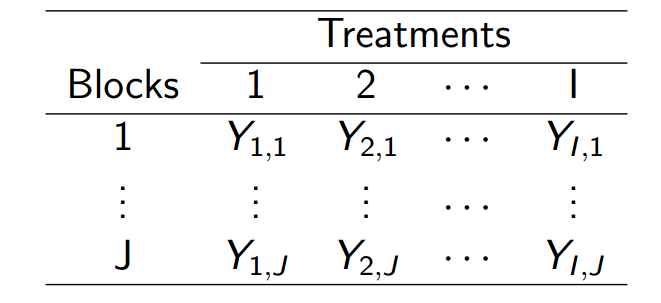
\includegraphics[width=0.5\linewidth]{fig/randomized-complete-block-design}
	\caption{Randomized Complete Block Design}
	\label{fig:randomized-complete-block-design}
\end{figure}

\subsection{Assumption}
\begin{itemize}
	\item The random variables $Y_{i,j}$'s all mutually independent
	\item For each fixed $(i, j)$, the random variable $Y_{i,j}$ follows continuous distribution $F_{ij}$.
	\item The distribution functions $F_{11}, \dots, F_{1k}, \dots, F_{n1}, \dots, F_{nk}$ are connected through the relationship
	\[F_{ij}(u) = F(u - \tau_i - \beta_j ), -\infty < u < \infty\]
	, for $i = 1, \dots, n$ and $j = 1, \dots, k$, where
	\begin{itemize}
		\item $F$ is a continuous distribution function with unknown median $\theta$.
		\item $\tau_i$ is the unknown additive treatment effect contributed by the $i$-th treatment.
		\item $\beta_j$ is the unknown additive effect contributed by block $j$.
	\end{itemize}
\end{itemize}

We can set up the model of each observation based on the assumptions.
\[Y_{ik} = \theta + \tau_i + \beta_j + \epsilon_{ij}\]
\begin{itemize}
	\item $\theta$: Overall median.
	\item $\tau_i$: the $i$-th treatment effect.
	\item $\beta_j$: the $j$-th block effect.
	\item $\epsilon_{ij}$: random error. iid from a continuous distribution with median 0.
\end{itemize}
\subsection{Hypothesis}
\begin{itemize}
	\item $H_0$: $\tau_1 = \cdots = \tau_I$, which means that $F_1 = \cdots F_I = F$.
	\item $H_1$: $\tau_1, \dots, \tau_I$ are not all equal.
\end{itemize}
\subsubsection{Rank Based Test Statistic, S}
To compute the Friedman statistic $S$, first order the  $I$ obervations from least to greatest separately within each of the $J$ blocks.

Let $r_{ij}$ denotes the rank of $Y_{ij}$ in this joint ranking of the $j$-th block, $i = 1, \dots, I$.

Let $R_i = \sum_{j=1}^{J} r_{ij}$, which is the sum of the within-blocks ranks received by the obervations in the $i$-th treatment.

Let $\bar{R}_i = \frac{R_i}{j}$, $i = 1, \dots, I$, which is the \textbf{average within-blocks rank} received by the observations in the $i$-th treatment. Note that the overall average rank is $(I + 1) / 2$.

\begin{figure}[H]
	\centering
	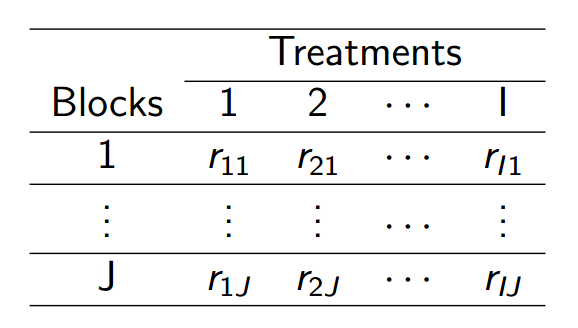
\includegraphics[width=0.45\linewidth]{fig/rank-schema}
	\caption{Rank Schema}
	\label{fig:rank-schema}
\end{figure}
\begin{figure}[H]
	\centering
	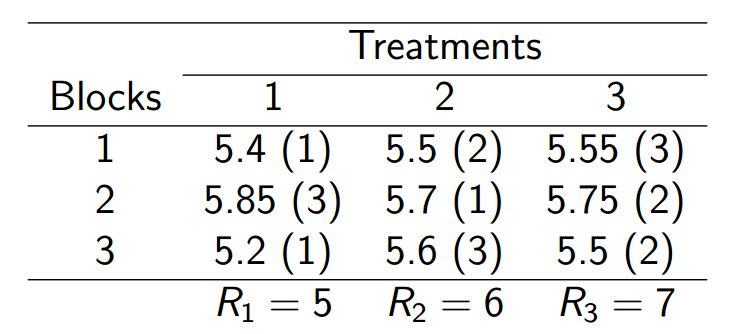
\includegraphics[width=0.45\linewidth]{fig/rank-example}
	\caption{Rank Example}
	\label{fig:rank-example}
\end{figure}

The Friedman statistic $S$ is given by 
\begin{align}
	S 
	&= (\frac{12}{I(I + 1)J} \sum_{i=1}^{I} R_i^2) - 3J(I+1)\\
	&= \frac{12J}{I(I+1)}\sum_{i=1}^{I} (\bar{R}_i - \frac{I + 1}{2})^2
\end{align}

Reject $H_0$ if $S > s_\alpha$, the upper $\alpha$ percentile for the null distribution of $S$.

\begin{lstlisting}[language=Python]
library(NSM3)
?cFrd
\end{lstlisting}

We can also use CTL to estimate the critical value.

Reject $H_0$ if $S \ge \chi_{I - 1,\alpha}^2$, as $J \rightarrow \infty$. $\chi_{I - 1,\alpha}^2$ is the upper $\alpha$ percentile point of a chi-square distribution with $I-1$ degree of freedom.

\subsection{Special Case: I = 2}
When $I = 2$, the data looks like paired-sample problem. Recall that \textbf{Wilcoxon's Rank Sum Test} is for location changes in paired-sample problem.
\begin{figure}[H]
	\centering
	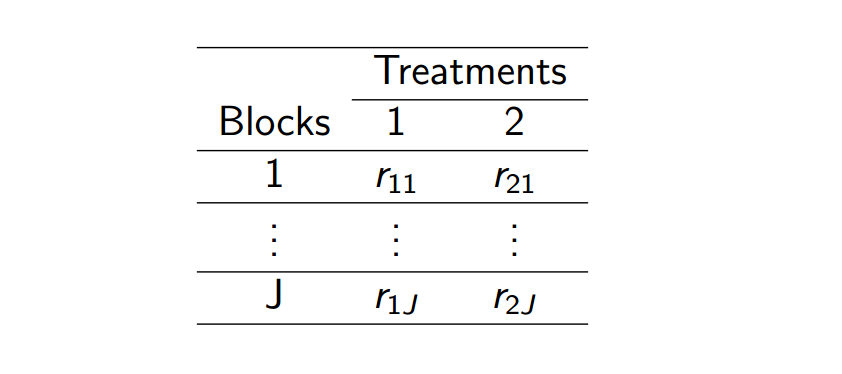
\includegraphics[width=0.7\linewidth]{fig/rank-example-i=2}
	\caption{Special Case, $I = 2$}
	\label{fig:rank-example-i2}
\end{figure}

In the following code, we use sign test, Friedman Rank Sum Test (CTL), and wilcox test to exam the difference of location between $X$ and $Y$. We have the $p$-values,
\begin{itemize}
	\item Sign Test: 0.1797
	\item Friedman Rank Sum Test (CTL): 0.0955807
	\item Friedman Rank Sum Test: 0.09558
	\item Wilcoxon signed rank exact test: 0.03906
\end{itemize}
We can tell that 
\lstinputlisting[language=R]{code/friedman.R}


\subsection{Multiple Comparison}
In a Friedman Test, if we reject the null hypothesis then we admit that there is treatment effect difference. Then we usually want to know that which one makes it different. So we want to xompare the $I (I - 1) / 2$ pairwise group differences.
\begin{itemize}
	\item Calculate $|R_u - R_v|$, $1 \le u < v \le I$.
	\item Decide $\tau_u \neq \tau_v$ if $|R_u - R_v| \ge r_\alpha$, otherwise decide $\tau_u = \tau_v$.
\end{itemize}

\lstinputlisting[language=R]{code/friedman-multiple.R}

\subsection{Extension: Mack-Skillings Test}
There can be more than one observation for some of the treatment-block combinations, i.e. replications in a given cell. To be more specific, we can have 
\begin{itemize}
	\item Some cells with no observation.
	\item Some cells with one observation.
	\item Some cells with replications.
\end{itemize}

The data can be represented with $I$ treatments and $J$ blocks. $n_{ij}$ subjects in the $(i, j)$-th cell. $N = \sum_{i=1}^{I} \sum_{j=1}^{J} n_{ij}$ observations. The Outcome $Y_{i,j,k}$, $k = 1, \dots, n_{ij}$.
\begin{figure}[H]
	\centering
	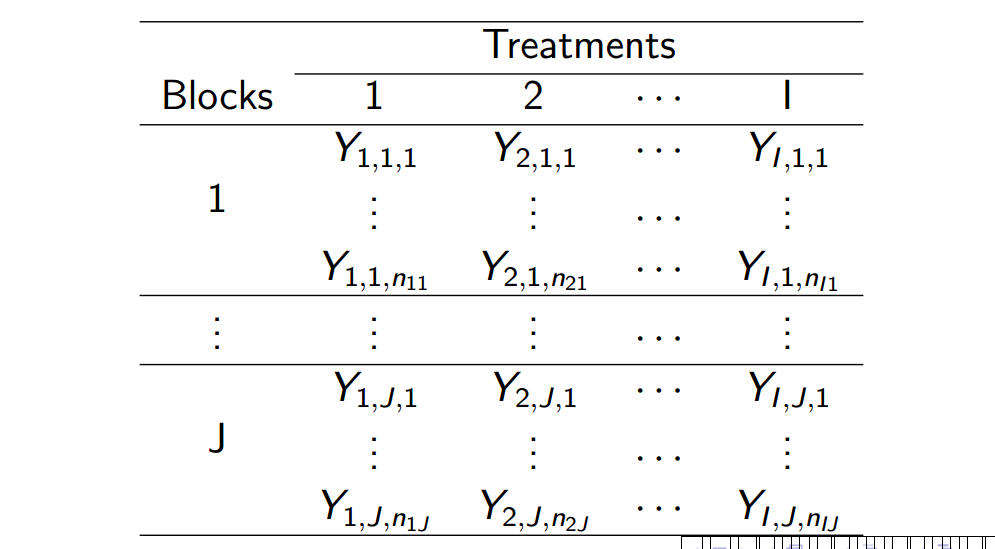
\includegraphics[width=0.7\linewidth]{fig/skillings-mack-data}
	\caption{Data Strucutre}
	\label{fig:skillings-mack-data}
\end{figure}

The assumptions
\begin{itemize}
	\item The random variables $Y_{i,j,k}$'s all mutually independent
	\item For each fixed $(i, j)$, the random variable $Y_{i,j,1}, \dots, Y_{i,j,n_{ij}}$ follow continuous distribution $F_{ij}$.
	\item The distribution functions $F_{11}, \dots, F_{1k}, \dots, F_{n1}, \dots, F_{nk}$ are connected through the relationship
	\[F_{ij}(u) = F(u - \tau_i - \beta_j ), -\infty < u < \infty\]
	, for $i = 1, \dots, n$ and $j = 1, \dots, k$, where
	\begin{itemize}
		\item $F$ is a continuous distribution function with unknown median $\theta$.
		\item $\tau_i$ is the unknown additive treatment effect contributed by the $i$-th treatment.
		\item $\beta_j$ is the unknown additive effect contributed by block $j$.
	\end{itemize}
\end{itemize} 

We can set up the model of each observation based on the assumptions.
\[Y_{ik} = \theta + \tau_i + \beta_j + \epsilon_{ijk}\]
\begin{itemize}
	\item $\theta$: Overall median.
	\item $\tau_i$: the $i$-th treatment effect.
	\item $\beta_j$: the $j$-th block effect.
	\item $\epsilon_{ijk}$: random error. iid from a continuous distribution with median 0.
\end{itemize}
The hypothesis are
\begin{itemize}
	\item $H_0$: $\tau_1 = \cdots = \tau_I$, which means that $F_{1j} = \cdots = F_{Ij} = F_j$, $j = 1, \dots, J$.
	\item $H_1$: $\tau_1, \dots, \tau_I$ are not all equal.
\end{itemize}

Example code
\lstinputlisting[language=R]{code/skillings-mack.R}
\end{document}
